\documentclass[UTF8]{ctexart}

\usepackage{subfiles}  

%下面的语句, 引入你的头部设置文件
\usepackage{C:/phpStorm_proj/02_myself_ID_EGO/+100_latex_all_math_sel/myPreamble} 
%必须是绝对路径,才能让各个tex在单独编译时使用到


\title{函数}


\begin{document}
	\tableofcontents % 生成目录
	\date{} % 若不写这句, 则默认也会渲染出日期, 所以我们要手动赋空值
	\maketitle  %这行代码, 让你前面的 title, author, date生效

\part{反函数}



\begin{tabular}{|l| l| }
	\hline
	函数f 是: 输入x, 输出y.
	 &  f(x自变量) = y因变量. \\	 
	\hline	
	
	反函数 $f^{-1}$ 是: 输入y, 输出x. 
	&  相当于时间倒流, 把原函数的功能倒过来.  \\
	& 就像线性代数中的"逆矩阵"变换功能. \\
	\hline
\end{tabular}
\\

``反函数"和``原函数", 图象关于直线 y=x 对称. \\


\begin{myEnvSample}
有函数 y = 3x+5, 即输入x, 输出y. 它可以变为: 
	\begin{align*}
		& 3x = y-5 \\
		& x = \frac{y-5} {3} 
	\end{align*}
	
	这样, 就是输入y, 输出x 的形式了, 即就变成了``反函数".
	
	但一般我们习惯于将输入值, 用x表示; 输出值 , 用y值表示, 所以上面的反函数, 就索性写成  $ y = \dfrac{x-5} {3} $, 但你不要混淆这里的x和y的意义. 这里的x是原y值, 这里的y是原x值.
\end{myEnvSample}






\part{初等函数}

\section{power function 幂函数:  $ y = x^{exp} $}

变量x 作为``底"的, 就是幂函数. 形如 $ y=x^2 $ , 格式是 $ y = x^{exp} $





\section{exponential function 指数函数:  $ y=base^x $}

变量x 在肩膀上做为次方来用的, 就是``指数函数". 形如 $ y=100(1+0.1)^x $. 格式是   $ y=base^x $. 其中, base \textgreater 0 并且 base≠1.

其实, ``投资回报率"终值计算公式 $ F=P(1+i)^n $, 就是指数函数. 如: $ y=100(1+0.1)^x $ 


\subsection{为什么 $base^0=1$ ?}

因为 $ 5^0 =5^{1-1}=\dfrac{5^1} {5^1} =1$

而 $ 0^0 =0^{1-1}=\dfrac{0^1} {0^1} $ ← 分母上不能为0, 所以无意义





\subsection{重要公式 $ \boxed{a^n=e^{n\cdot \ln a}}$}

证明过程, 我们倒过来做: \\

\begin{myEnvSample}
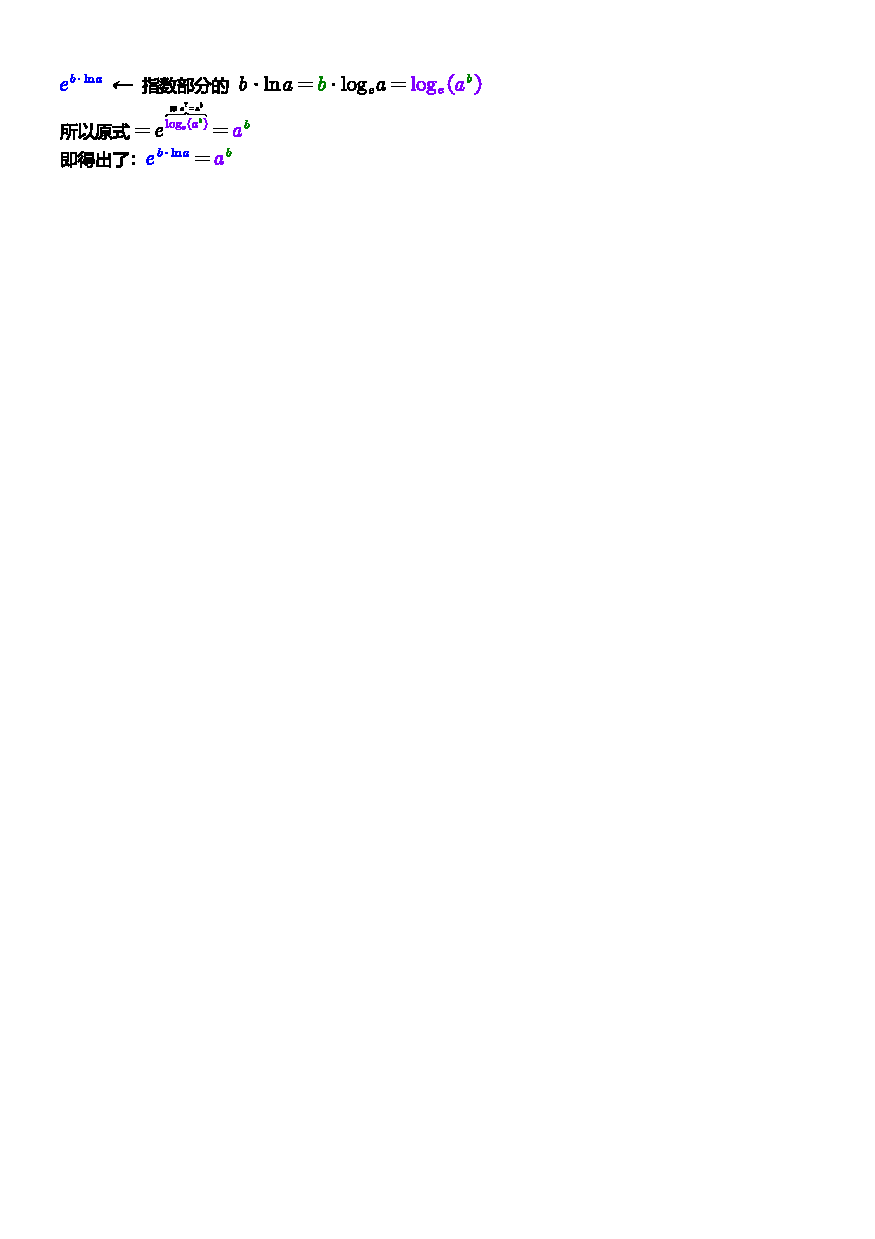
\includegraphics[width=0.55\textwidth]{/0034.pdf} \\

即: \\
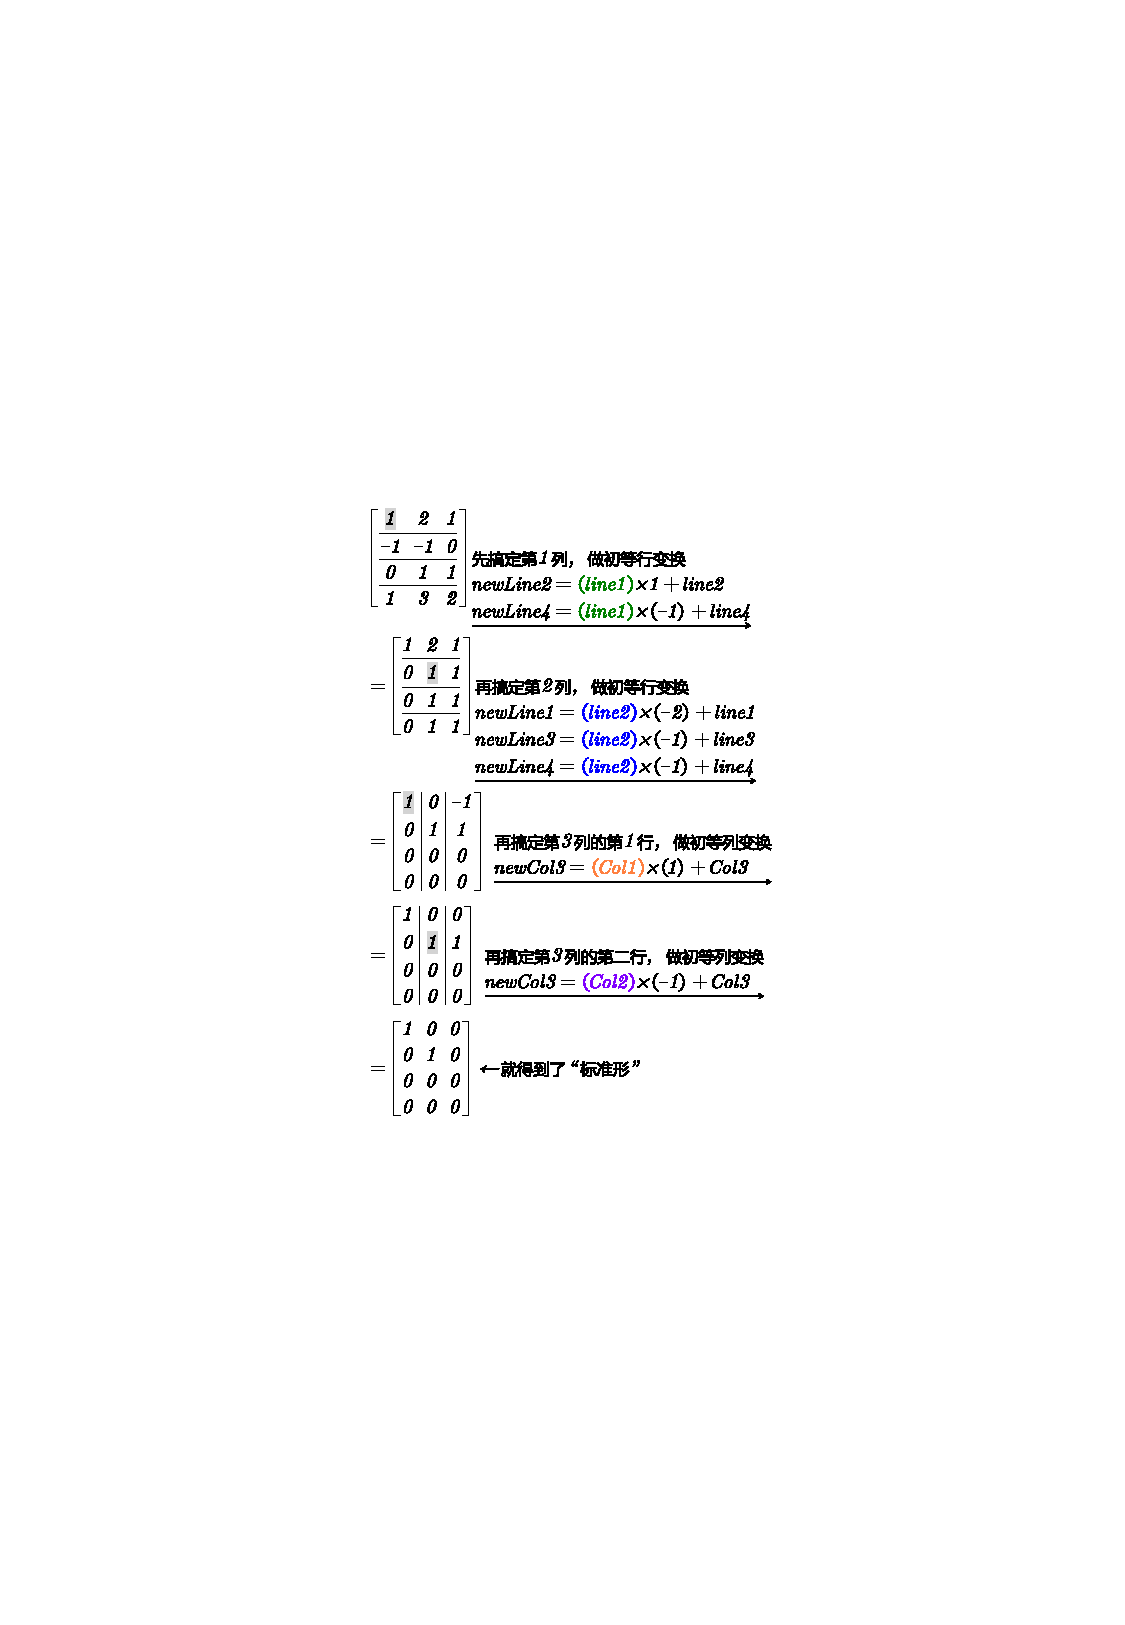
\includegraphics[width=0.27\textwidth]{/0035.pdf}
\end{myEnvSample}

记忆法: 把底数(a)换成e, 把指数(n)换成: 原指数后面再乘个``ln底" (n × ln a).  即 $a^n=e^{n\cdot \ln a}$




\section{Logarithmic function 对数函数:  $ \log _{\text{底}}\text{幂}=\text{指} $}

- 底数 Base Number

- 指数 Exponent

- 幂 Power

有: $\text{底}^{\text{指}}=\text{幂}$,  则: → $ \log _{\text{底}}\text{幂}=\text{指} $ \\


- $\log _{10}\text{幂}=\lg\text{幂}$

- $\log _e\text{幂}=\ln\text{幂}$ \\

显然, 就有:


\subsection{$\text{底}^{\log _{\text{底}}\text{幂}}=\text{幂}$}

即 
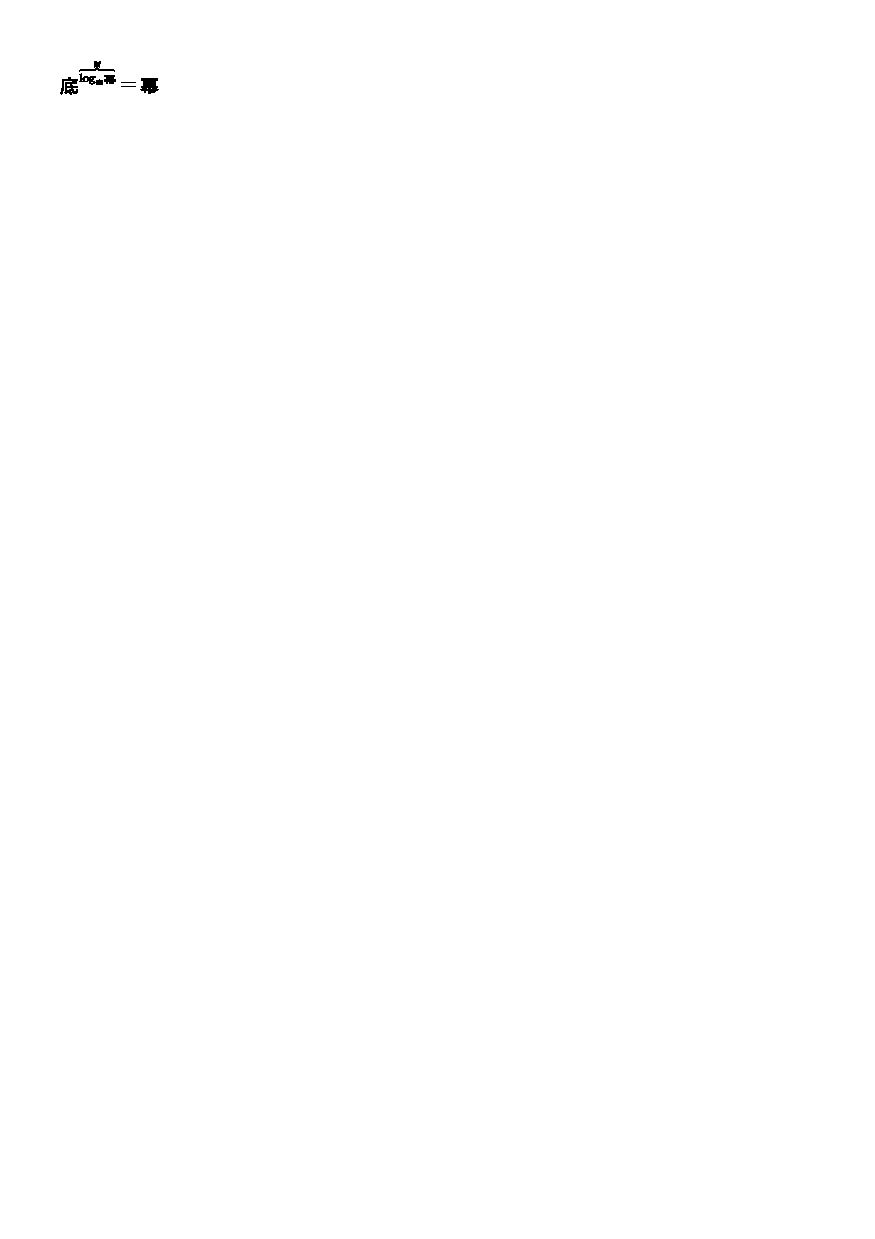
\includegraphics[width=0.12\textwidth]{/0028.pdf} \\


\begin{myEnvSample}
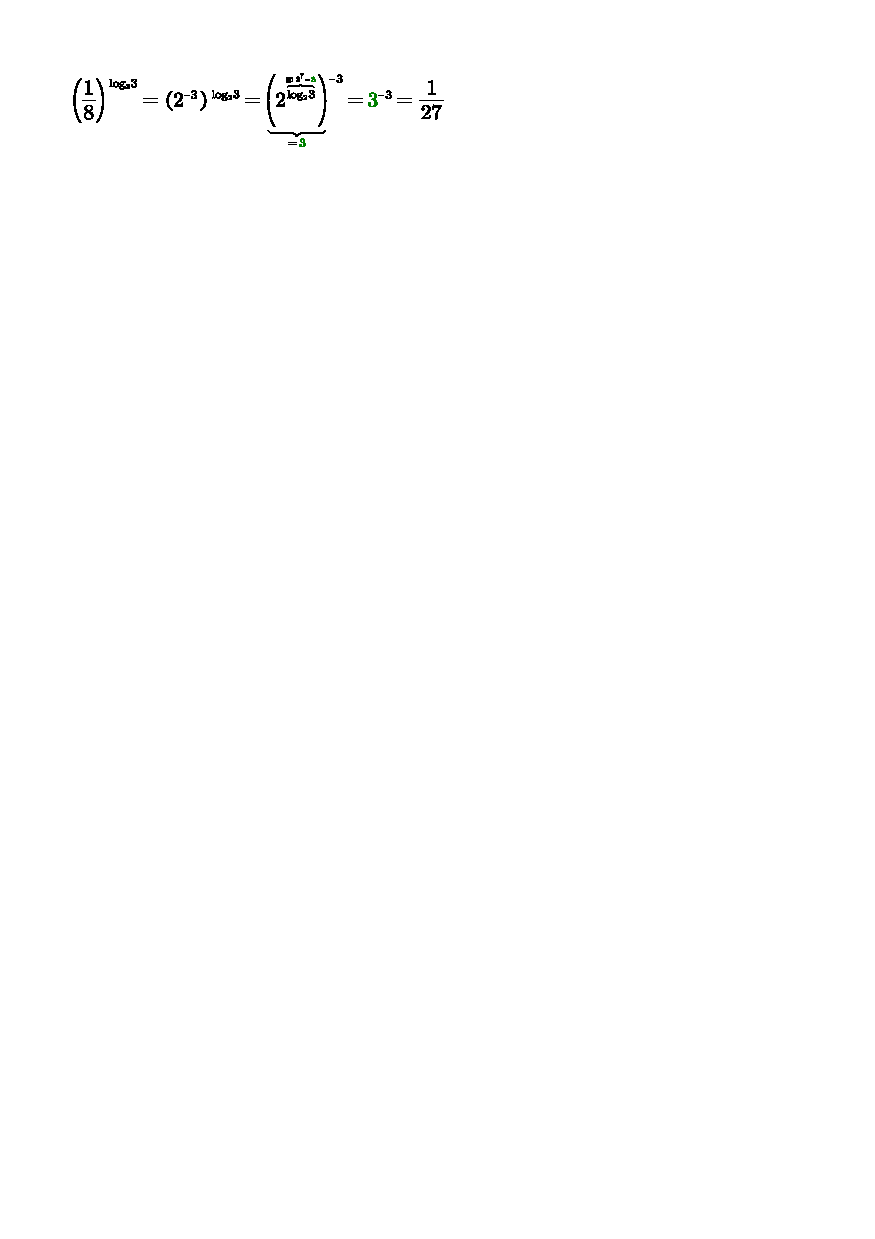
\includegraphics[width=0.5\textwidth]{/0032.pdf}
\end{myEnvSample}


\dotfill


\subsection{$\log _{\text{底}}\text{底}^{\text{指}}=\text{指}$}

即 
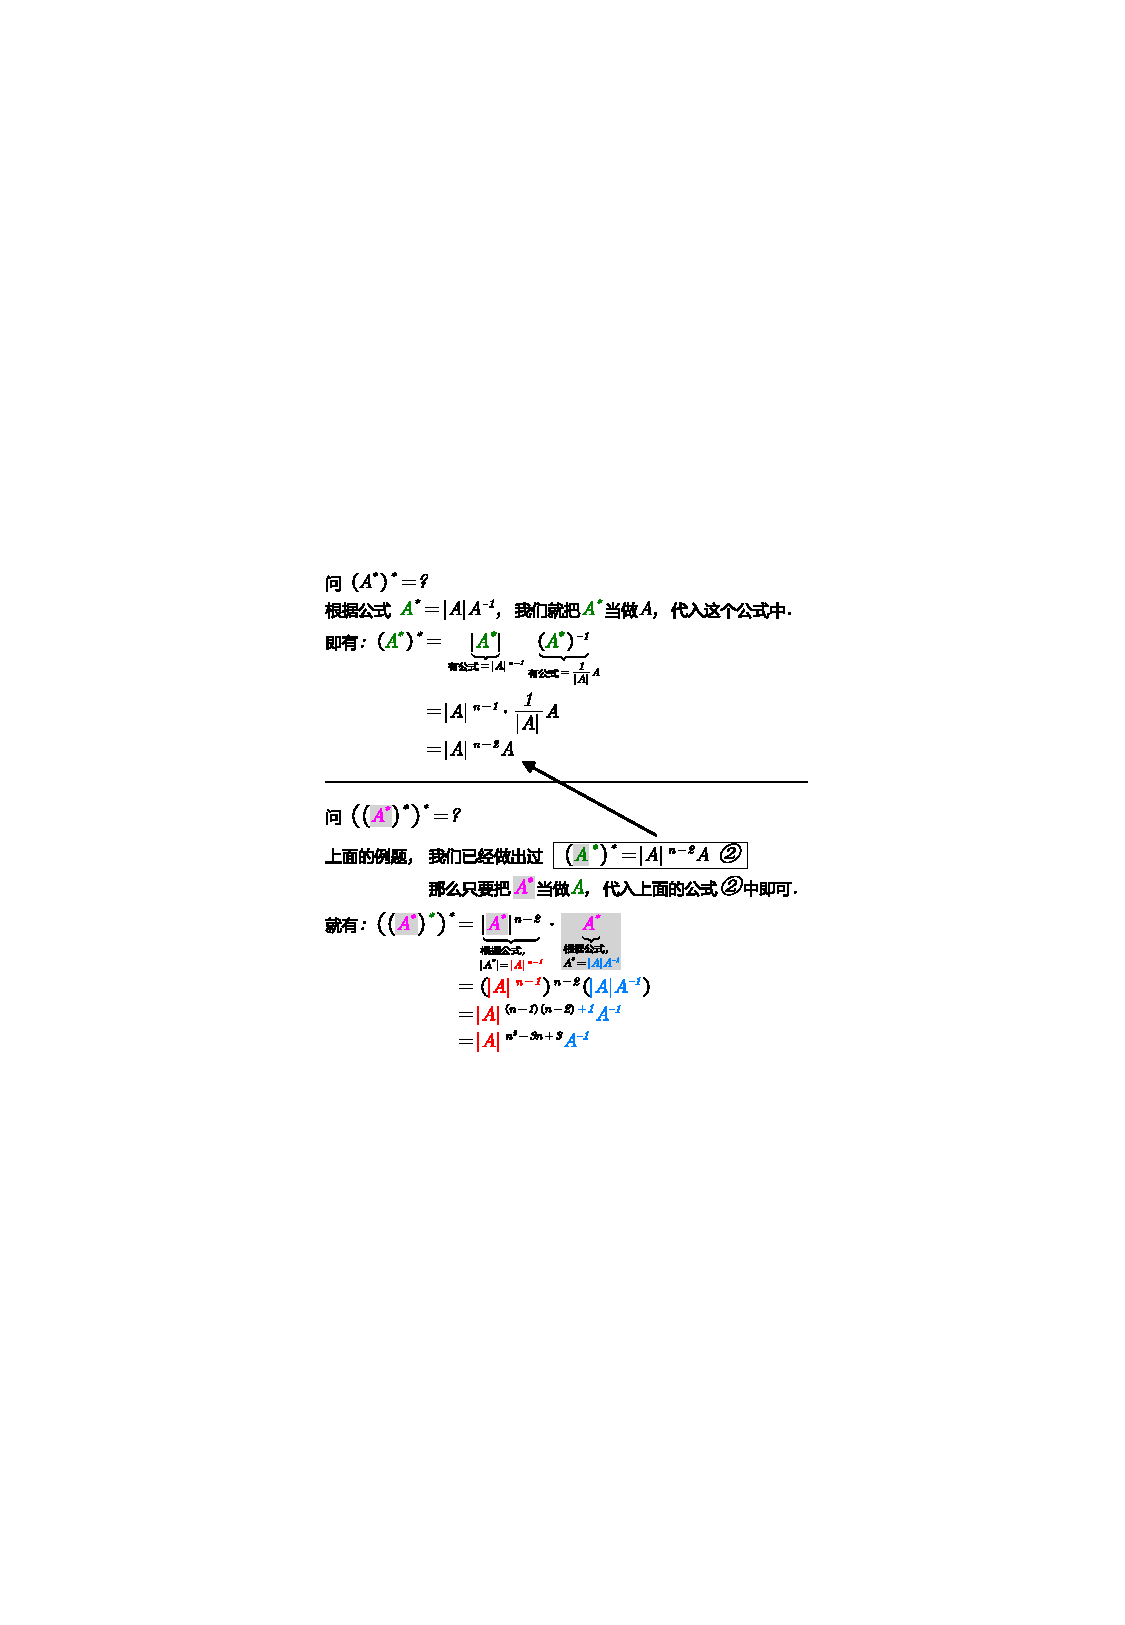
\includegraphics[width=0.13\textwidth]{/0029.pdf}


\dotfill



\subsection{$\log _{\text{底}}\left( \frac{\text{幂}1}{\text{幂}2} \right) =\log _{\text{底}}\text{幂}1-\log _{\text{底}}\text{幂}2$}

即 : \\
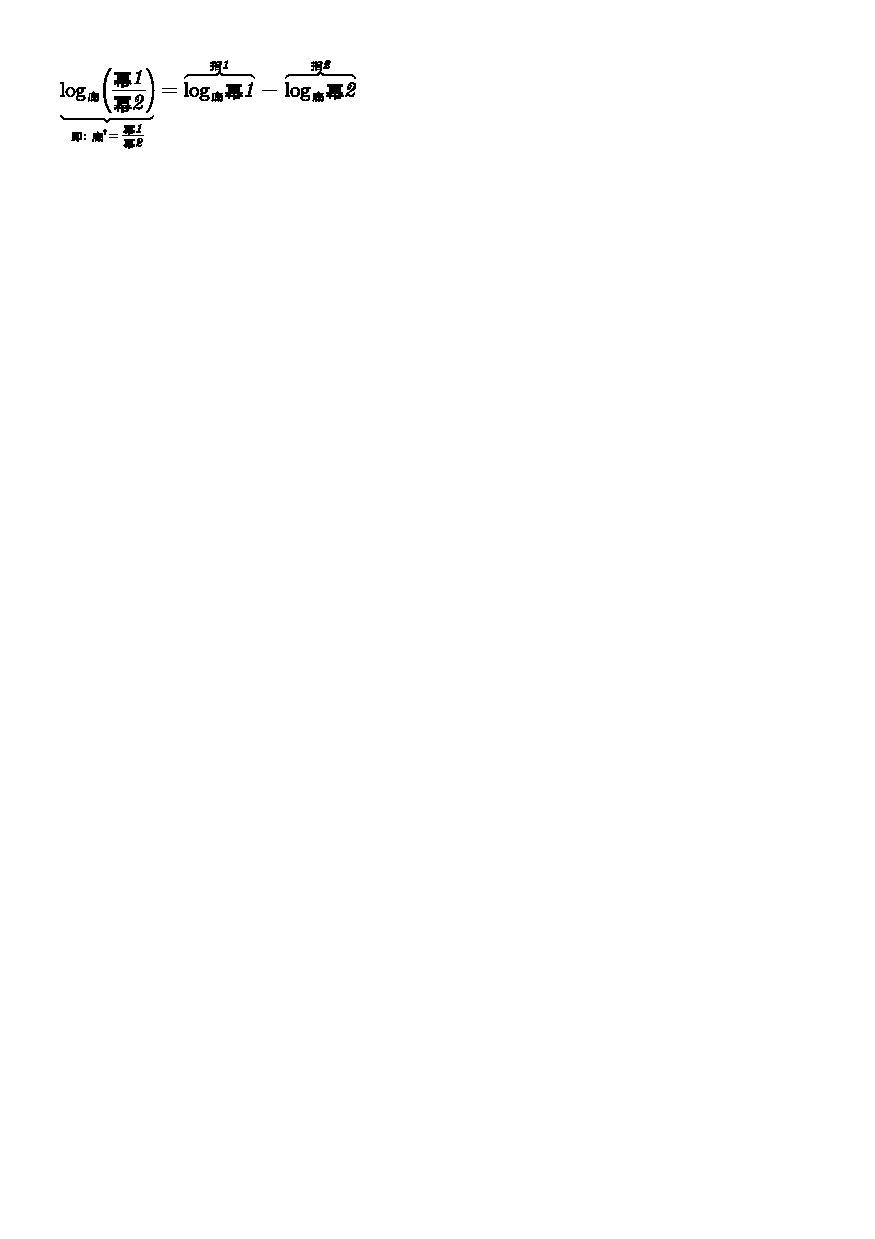
\includegraphics[width=0.4\textwidth]{/0030.pdf}


反过来, 即是:  $\log _{\text{底}}\text{幂}1-\log _{\text{底}}\text{幂}2=\log _{\text{底}}\left( \dfrac{\text{幂}1}{\text{幂}2} \right) $


\dotfill


\subsection{$\log _{\text{底}}\text{幂}1+\log _{\text{底}}\text{幂}2=\log _{\text{底}}\left( \text{幂}1\cdot \text{幂}2 \right) $}





\dotfill

\subsection{$\boxed{\log _{\text{原底}}\text{幂}=\dfrac{\log _{\text{任意底}}\text{幂}}{\log _{\text{任意底}}\text{原底}}}$ ← 这个就是 ``换底公式"}

由换底公式, 可以推导出以下一些常用的结论: \\

→  $\log _{\text{原底}}\text{幂}=\dfrac{\log _{\text{幂}}\text{幂}}{\log _{\text{幂}}\text{原底}}=\dfrac{1}{\log _{\text{幂}}\text{原底}}$ 
← 看一头一尾, 即就有: $\boxed{\log _{\text{底}}\text{幂}\cdot \log _{\text{幂}}\text{底}=1}$
\\

→ $ \boxed{\log _{\text{底}1}\text{幂}1\cdot \log _{\text{幂}1}\text{幂}2=\log _{\text{底}1}\text{幂}2 }$

即: \\
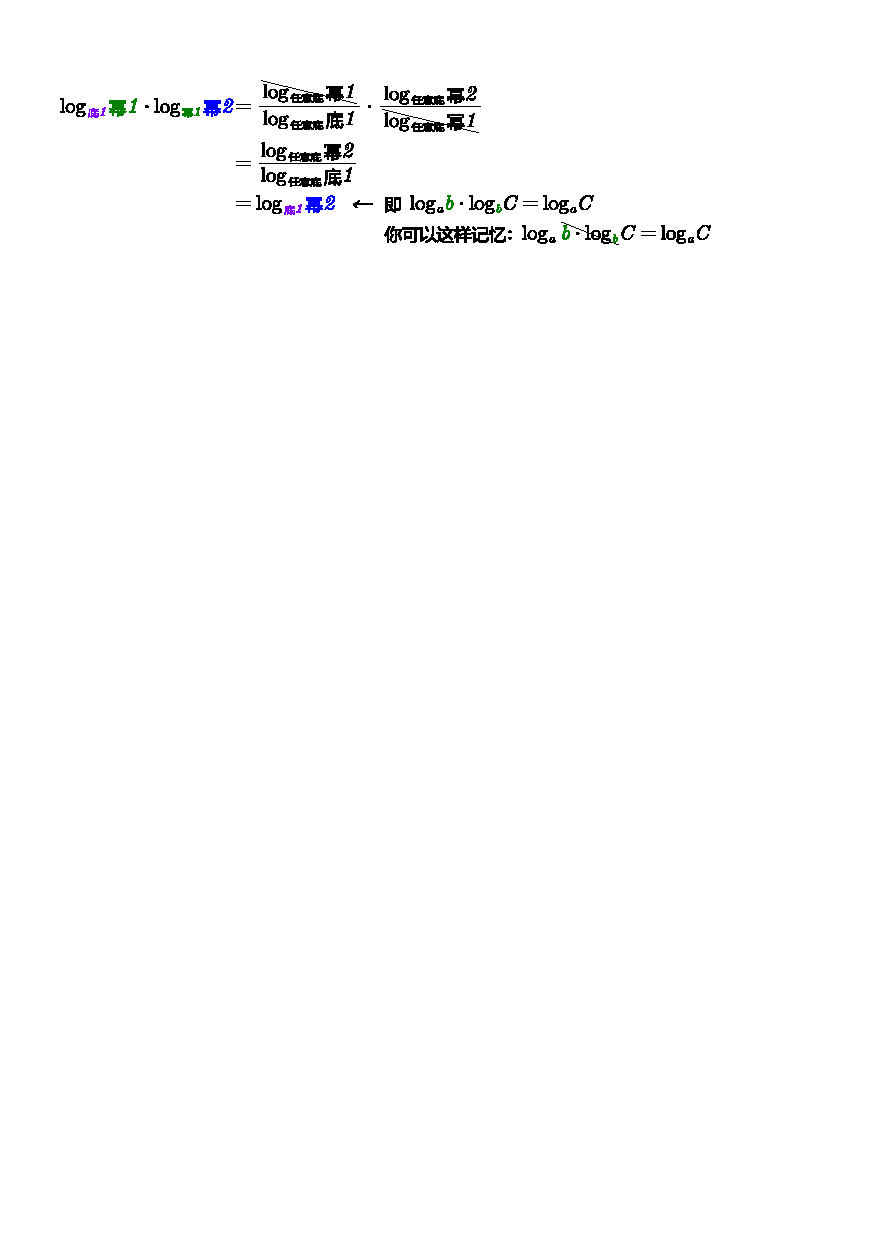
\includegraphics[width=0.8\textwidth]{/0031.pdf}



→ $ \boxed{\log _{\text{原底}}\text{幂:\ }\rightarrow \text{根据换底公式,有}=\frac{\log _{10}\text{幂}}{\log _{10}\text{原底}}=\frac{\lg\text{幂}}{\lg\text{原底}}
}$

即有, 例如: $\log _a2=\dfrac{\lg 2}{\lg a} $



\dotfill



\subsection{$\log _{a^n}b^m=\frac{m}{n}\log _ab $}

← 简单记忆法: 把 m 和n, 上下保持不动, 直接向左平移到 log 外面去就行了. \\

\begin{myEnvSample}
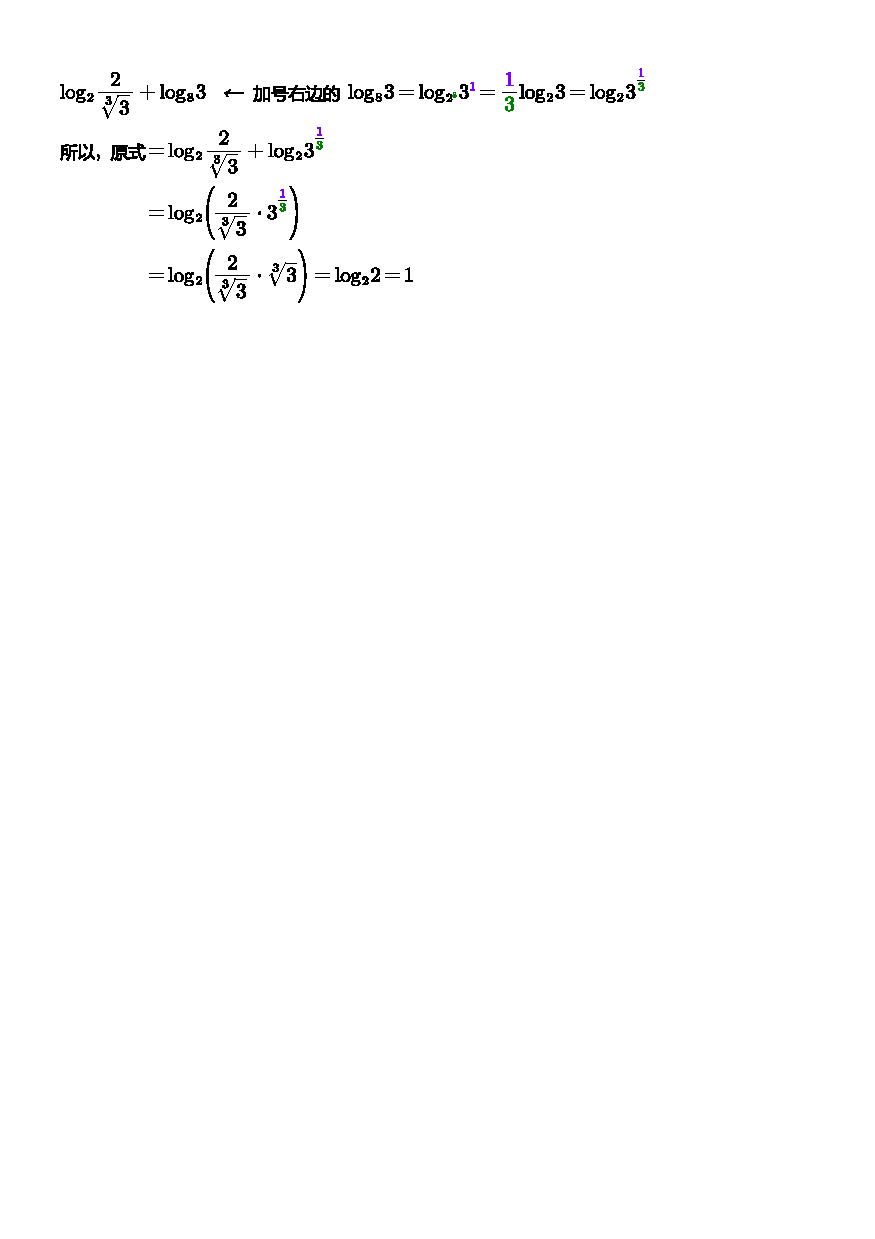
\includegraphics[width=0.75\textwidth]{/0033.pdf}
\end{myEnvSample}



这个公式可以推导出: \\


→ $\log _{\text{底}}M^n=\log _{\text{底}^1}M^n=\frac{n}{1}\log _{\text{底}}M=n\cdot \log _{\text{底}}M $

→ $ \log _{a^n}b^n=\frac{n}{n}\log _ab=\log _ab$

→ $\log _{a^n}a^m=\frac{m}{n}\log _aa=\frac{m}{n}\cdot 1=\frac{m}{n} $


→ $\ln a^b=\log _{e^1}a^b=\frac{b}{1}\log _ea=b\ln a $





\section{trigonometric function 三角函数:  $ y=base^x $}

\subsection{sin \& arcSin}





\subsection{cos \& arcCos}



\subsection{tan \& arcTan}




\subsection{cot \& arcCot}




\subsection{sec \& arcSec}




\subsection{csc \& arcCsc}



\end{document}

